\documentclass[journal]{IEEEtran}
\usepackage[utf8]{inputenc}
\usepackage[T1]{fontenc}
\usepackage{amsmath,amssymb}
\usepackage{graphicx}
\usepackage{booktabs}
\usepackage{multirow}
\usepackage{array}
\usepackage{url}
\usepackage[hidelinks]{hyperref}
\usepackage{cite}
\usepackage{textcomp}
\newcommand{\wf}{W-F1}
\newcommand{\kbar}{\bar{k}}
\newcommand{\TODO}[1]{\textbf{[#1]}}

\begin{document}

\title{When Does Conversational Context Help Emotion Recognition?\\A Hardness-Stratified Study of Adaptive Context in Multimodal ERC with a Pre-Specified Decision Rule}

\author{Sudipta~Bhattacharya,~\IEEEmembership{Member,~IEEE}%
\thanks{S.~Bhattacharya is with the IEM Centre of Excellence for Cloud Computing and IoT, Department of CSE (AIML) and CSBS, Institute of Engineering and Management, School of University of Engineering \& Management, Kolkata 700091, India (e-mail: bhattacharya.sudipta@gmail.com).}%
\thanks{Manuscript received November 2026.}}

\markboth{IEEE Transactions on Affective Computing}{Bhattacharya: When Does Conversational Context Help Emotion Recognition?}

\maketitle

\begin{abstract}
Emotion recognition in conversation (ERC) models read a fixed number of preceding utterances for every target utterance, yet it is widely assumed that only the ambiguous utterances need that context. We test this assumption directly, under a decision rule specified before the decisive runs, on IEMOCAP (speech + text, 6 classes, Sessions 1--4 / 5), MELD (speech + text, 7 classes) and EmoryNLP (text, 7 classes), using frozen WavLM-Large and RoBERTa-base encoders with a 0.32\,M-parameter head so that every effect is attributable to the context mechanism rather than to encoder fine-tuning. An instance-hardness score $h$---the normalised label entropy of an utterance's $K$ nearest training-fold neighbours in embedding space, computed without the target's own label, dialogue or speaker---stratifies the corpus. Three results follow. (1)~Context is worth $+8.4$ weighted-F1 (\wf) on IEMOCAP ($58.8 \pm 0.8 \rightarrow 67.2 \pm 0.8$ over 5 seeds) and nothing on MELD ($62.5 \rightarrow 62.3$), and on IEMOCAP the gain rises with hardness: $+4.8$ \wf{} in the easiest quartile, $+9.8$ and $+8.2$ in the middle two, $+11.2$ in the hardest (relative error reduction $15 \rightarrow 23\%$). (2)~Despite this, a learned policy that predicts how much context each utterance needs---trained on an oracle of sufficient context and evaluated against random assignment at the same mean context, fixed windows and a posterior-entropy policy---never beats a fixed 8-turn window ($65.5$ vs $67.2$ \wf; paired-bootstrap 95\% CI of fixed-8 minus policy $[+0.1, +3.3]$) and is indistinguishable from random assignment at matched mean context ($65.5 \pm 1.7$ vs $64.8 \pm 2.1$ when both are trained under their own assignment; $66.3$ vs $66.5$ for one window-agnostic model evaluated both ways). The sufficient-context oracle explains why: 32--42\% of utterances are resolved without context, 35--44\% are not resolved at any context length, and $h$ ranks difficulty, not context-dependence. (3)~$h$ is not an estimate of human ambiguity: its Spearman correlation with inter-annotator disagreement on the 1{,}622 IEMOCAP Session-5 test utterances (pooled over 5 seeds) is $0.04$ (partial, given model entropy: $0.02$), against a pre-committed threshold of $0.15$. Hardness-conditioned gating, curriculum weighting with either sign of $\lambda$, and the choice of context head all fall within seed noise. We release code, cached embeddings and per-seed results. The findings argue for using hardness to stratify ERC evaluation and to decide \emph{whether} a corpus rewards context, not to decide per utterance how much context to read.
\end{abstract}

\begin{IEEEkeywords}
Emotion recognition in conversation, multimodal affective computing, instance hardness, conversational context, self-supervised speech representations, pre-specified evaluation, negative results.
\end{IEEEkeywords}

\IEEEpeerreviewmaketitle

\section{Introduction}
\IEEEPARstart{E}{very} emotion-recognition-in-conversation (ERC) system since DialogueRNN~\cite{majumder2019dialoguernn} reads the dialogue history before classifying an utterance, and every one of them reads the \emph{same} amount of history for every utterance---a window, a whole dialogue, or a graph over all turns. The intuition that motivates context is nevertheless instance-specific: a flat ``okay'' needs the previous turns, a shouted insult does not. This gap between the motivation (some utterances need context) and the practice (all utterances get it) has produced a line of adaptive-context proposals---emotion-shift gates, learned window sizes, dynamic graph edges~\cite{bansal2022shapes}---whose reported gains over a well-tuned fixed window are small, rarely accompanied by variance estimates, and to our knowledge never compared against the two baselines that would falsify them: \emph{random} assignment of the same mean context and an \emph{oracle} that knows how much context each utterance actually needed.

This paper asks the question directly, and commits in advance to what would count as an answer. We define an instance-hardness score $h(t)$ for every utterance from frozen self-supervised embeddings alone: the normalised label entropy of its $K$ nearest training-fold neighbours, with the utterance itself, its dialogue and (on IEMOCAP) its speaker excluded. Because $h$ never reads the target label, it is identical at training and test time and can stratify any result table without leakage. We then build a window-agnostic multimodal ERC head on frozen WavLM-Large~\cite{chen2022wavlm} and RoBERTa-base~\cite{liu2019roberta} and run three pre-specified tests: \emph{does} context help, \emph{for whom} does it help, and can a policy that predicts per-utterance context length---trained on an oracle of sufficient context---beat a fixed window at equal or lower mean context. A fourth test asks whether $h$ tracks human disagreement, which would make it a classifier-free estimate of ambiguity.

The outcome is mixed in a way that is informative. Context is worth $+8.4$ \wf{} on IEMOCAP and nothing on MELD, and on IEMOCAP the gain rises with $h$ (Section~\ref{sec:strat}): the hardest quartile gains $2.3\times$ the absolute \wf{} of the easiest and removes 23\% of its errors against 15\%, with the two middle quartiles indistinguishable from each other. Yet the learned policy does not convert this into accuracy or into context savings. It is indistinguishable from random assignment at the same mean context and loses $1.7$ \wf{} to the fixed 8-turn window (Section~\ref{sec:policies}). The oracle shows why: roughly 40\% of utterances need no context and roughly 40\% are never resolved at any length, and a predictor of sufficient context cannot separate the two from the utterance embedding (Section~\ref{sec:discussion}). $h$ is also uncorrelated with inter-annotator disagreement ($\rho = 0.04$, Section~\ref{sec:conf}). Both pre-committed success criteria for a method claim therefore fail, and we report the study as an analysis.

The contributions are:
\begin{enumerate}
\item \textbf{A label-free hardness score for ERC and the first hardness-stratified measurement of context gain.} On IEMOCAP (speech + text) the benefit of eight turns of context rises from $+4.8$ \wf{} in the easiest quartile to $+11.2$ in the hardest ($+9.8$ and $+8.2$ in between); on MELD it is flat and near zero in every quartile (Table~\ref{tab:strat}, Fig.~\ref{fig:quartile}).
\item \textbf{A pre-specified negative result on adaptive context length,} with the baselines the literature omits: at matched mean context a hardness-guided policy ties random assignment ($65.5 \pm 1.7$ vs $64.8 \pm 2.1$ \wf{} trained; $66.3$ vs $66.5$ at inference), and at its dev-selected operating point it trails a fixed 8-turn window ($65.5$ vs $67.2$; paired-bootstrap 95\% CI of fixed-8 minus policy $[+0.1, +3.3]$). A sufficient-context oracle (Table~\ref{tab:oracle}) explains the failure as a property of the data, not of the predictor.
\item \textbf{A negative result on hardness as an ambiguity estimate:} on the 1{,}622 IEMOCAP Session-5 test utterances, each carrying three evaluator votes, $\rho(h,\text{disagreement}) = 0.04$ and the partial correlation given model entropy is $0.02$; model entropy itself reaches only $0.11$.
\item \textbf{A reproducible frozen-encoder baseline}---$67.2$ \wf{} on 6-class IEMOCAP (Ses05), $62.5$ on MELD, $35.1$ on EmoryNLP with 0.32\,M trainable parameters, 5 seeds, paired-bootstrap CIs, inner-dev model selection and a speaker-independent IEMOCAP replication (LOSO $62.1$)---with code, cached embeddings and per-seed results released.
\end{enumerate}

Section~\ref{sec:related} places the work; Section~\ref{sec:method} defines the score, the head and the policy; Section~\ref{sec:protocol} gives the protocol and the decision rule written before the multimodal runs; Section~\ref{sec:results} reports results; Section~\ref{sec:discussion} discusses the mechanism; Sections~\ref{sec:limits}--\ref{sec:conclusion} close.

\section{Related Work}\label{sec:related}
\textbf{Self-supervised speech and text encoders.} wav2vec~2.0~\cite{baevski2020wav2vec}, HuBERT~\cite{hsu2021hubert} and WavLM~\cite{chen2022wavlm} replaced hand-crafted acoustic features in speech emotion recognition; on SUPERB-ER~\cite{yang2021superb} a frozen WavLM-Large with a light head is within a few points of full fine-tuning, and emotion2vec~\cite{ma2024emotion2vec} and EmoBox~\cite{ma2024emobox} show that layer-weighted frozen features are a strong, cheap and reproducible basis. We follow that practice deliberately: with encoders frozen, every effect we measure belongs to the context mechanism, and the embeddings can be cached once and released.

\textbf{Context modelling in ERC.} DialogueRNN~\cite{majumder2019dialoguernn} and DialogueGCN~\cite{ghosal2019dialoguegcn} introduced recurrent and graph models of the dialogue; COSMIC~\cite{ghosal2020cosmic}, DAG-ERC~\cite{shen2021dagerc} and DialogXL~\cite{shen2021dialogxl} refined how far and in which direction context flows; multimodal systems---MMGCN~\cite{hu2021mmgcn}, DialogueCRN~\cite{hu2021dialoguecrn}, MM-DFN~\cite{hu2022mmdfn}, COGMEN~\cite{joshi2022cogmen}, CORECT~\cite{nguyen2023corect}, SDT~\cite{ma2024sdt}, UniMSE~\cite{hu2022unimse}, MultiEMO~\cite{shi2023multiemo}---add fusion and distillation on top. All read the same context for every utterance; the few adaptive proposals---emotion-shift modelling~\cite{bansal2022shapes}, shift-aware curricula~\cite{yang2022hybrid}, dynamic graph edges---report gains of 0.5--1.5 \wf{} without seed variance or a matched-context control. Independent re-runs put published numbers in perspective: MultiEMO's reported $72.8$ \wf{} on IEMOCAP reproduces at $66.9 \pm 2.0$ under a common protocol~\cite{dutta2026mister}. LLM-based ERC (InstructERC~\cite{lei2023instructerc}) reaches $71.4 / 69.2$ on IEMOCAP / MELD by fine-tuning a 7\,B model; it is an upper reference, not a comparable budget.

\textbf{Instance hardness.} Smith et al.~\cite{smith2014instance} defined instance hardness through $k$-disagreeing neighbours and showed it transfers across learners; Lorena et al.~\cite{lorena2019complex} survey such measures. In affective computing, Lotfian and Busso~\cite{lotfian2019curriculum} used \emph{annotator} disagreement as a curriculum signal and Hybrid Curriculum Learning~\cite{yang2022hybrid} used an emotion-shift difficulty for ERC. Dataset cartography~\cite{swayamdipta2020cartography} maps instances by training dynamics; our score is instead computed from frozen embeddings, before any classifier is trained. Loss re-weighting by difficulty has both signs in the literature---focal loss~\cite{lin2017focal} up-weights hard examples, AUM~\cite{pleiss2020aum} and confident learning~\cite{northcutt2021confident} down-weight or remove them as likely label noise. We evaluate both signs and find neither matters here. We are not aware of prior ERC work that uses a label-free hardness score to decide how much context to read, or to stratify the measured gain of context.

\textbf{Calibration and selective prediction.} ERC systems are rarely evaluated for calibration; we report ECE~\cite{guo2017calibration} and the area under the risk--coverage curve~\cite{geifman2019aurc} and test whether $h$ adds to the model's own confidence as a rejection signal.

\section{Method}\label{sec:method}
The system has three parts (Fig.~\ref{fig:arch}): a hardness score computed once from frozen embeddings; a multimodal context head that classifies a target utterance from a masked window of up to $K_{\max} = 8$ preceding utterances; and a context-length predictor $g$ trained on an oracle of sufficient context. Everything below the encoders is 0.32\,M parameters (0.47\,M for the GRU head).

\begin{figure*}[t]\centering
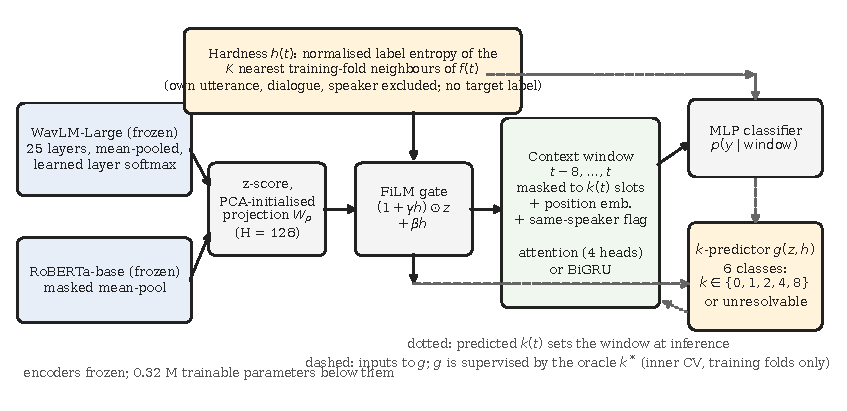
\includegraphics[width=\textwidth]{figures/fig1_architecture.pdf}
\caption{Hardness score, window-agnostic context head and context-length predictor. Encoders are frozen; the hardness score is computed once from the frozen embeddings and never reads the target label; the $k$-predictor is supervised by an oracle of sufficient context computed inside the training folds.}\label{fig:arch}
\end{figure*}

\subsection{Frozen encoders and fusion}
For utterance $t$, WavLM-Large~\cite{chen2022wavlm} gives 25 hidden-layer outputs, each mean-pooled over time (1024-d); a learned softmax over layer weights produces one acoustic vector $a(t)$. RoBERTa-base~\cite{liu2019roberta} gives a masked mean-pooled text vector $x(t)$ (768-d). Both are z-scored with training-fold statistics. The fused vector $f(t) = [a(t); x(t)]$ is projected to $H = 128$ dimensions by a linear map initialised from the PCA of the training fold and then trained. Encoders are never updated. A corpus without audio (EmoryNLP) receives a zero acoustic branch.

\subsection{Instance hardness}
Let $N_K(t)$ be the $K$ cosine-nearest neighbours of $f(t)$ among \emph{training-fold} utterances, excluding $t$ itself, every utterance from $t$'s dialogue and, on IEMOCAP, every utterance by $t$'s speaker. With $\hat p_c = |\{i \in N_K(t): y(i) = c\}| / K$,
\begin{equation}
h(t) = -\frac{1}{\log C}\sum_{c=1}^{C} \hat p_c \log \hat p_c, \qquad h(t) \in [0,1].
\end{equation}
$h$ is 0 when all neighbours share a label and 1 when they are uniformly spread. It never reads $y(t)$, so it is the same quantity for training, development and test utterances; it is recomputed inside every fold so that no held-out label enters it; $K \in \{5, 10, 20\}$ is selected on the inner development split ($K = 5$ or $10$ on every primary split; two IEMOCAP LOSO folds selected $K = 20$). The acoustic part of $f(t)$ used for the neighbour search is the mean over WavLM layers, since the learned layer weights do not exist before training. We stress what $h$ measures: how \emph{mixed} the labels of acoustically-and-lexically similar utterances are---a property of the class boundary near $t$, not of $t$'s dialogue.

\subsection{Hardness-conditioned representation}
The projected vector is modulated by $h$ through a FiLM gate~\cite{perez2018film}, $z(t) = (1 + \gamma h(t)) \odot W_p^{\top} \tilde f(t) + \beta h(t)$, with $\gamma, \beta \in \mathbb{R}^H$ learned. Ablations replace the gate by scalar concatenation $[z; h]$, by a \emph{random} gate ($h$ permuted within each split, matched marginal) and by no gate.

\subsection{Context head}
The window for $t$ holds the slots $t-K_{\max} \ldots t$; slots beyond the dialogue start or beyond the selected length $k(t)$ are masked. Each slot receives $z$, a learned position embedding and a same-speaker/other-speaker embedding. The default head is one multi-head attention layer (4 heads)~\cite{vaswani2017attention} with a learned query over the unmasked slots; the alternative is a speaker-aware bidirectional GRU whose state at the target slot is read. The context vector is added to $z(t)$ and classified by a two-layer MLP. The head is \emph{window-agnostic}: the same parameters serve any $k$, which is what makes fixed-$k$, random-$k$ and adaptive-$k$ policies comparable with one architecture.

\subsection{Oracle of sufficient context}\label{sec:oracle}
Inside each training fold, a 5-fold inner cross-validation trains fixed-window classifiers for every $k \in \{0, 1, 2, 4, 8\}$ with three seeds and records, for each held-out utterance, the seed-averaged margin $m_k(t) = p(y(t)) - \max_{c \neq y} p(c)$. The oracle is $k^*(t) = \min\{k : m_{k'}(t) > \tau \ \forall k' \geq k\}$, $\tau = 0.10$; an utterance never classified with margin above $\tau$ is labelled \emph{unresolvable}. Test utterances have no $k^*$; the oracle exists to supervise $g$ and to describe the data (Table~\ref{tab:oracle}). Two properties of this definition should be read into Table~\ref{tab:oracle}: the inner models (15 epochs, 3 seeds) are weaker than the main models (30 epochs, early stopping), which inflates the \emph{unresolvable} share, and the ``for all $k' \geq k$'' clause makes $k^* = 8$ rare by construction, since an utterance helped by eight turns but hurt by four is assigned $k^* = 8$ only if the margin holds at 8 alone.

\subsection{Adaptive context policy}\label{sec:policy}
$g(z(t), h(t))$ is a two-layer MLP over six classes (five lengths and \emph{unresolvable}) trained with cross-entropy on $k^*$ jointly with the classifier (weight 0.3). Training pass~1 draws $k$ uniformly from $\{0,1,2,4,8\}$ for every utterance at every access, so the classifier is window-agnostic and $g$ sees all lengths. The decision rule at inference is: predicted \emph{unresolvable} $\rightarrow k = 8$; otherwise the smallest $k$ with predicted $P(k^* \leq k \mid \text{resolvable}) \geq \tau_k$, $\tau_k \in \{0.5, 0.7, 0.9\}$ selected on the inner development split. Pass~2 retrains the classifier under its own policy, i.e.\ with the predicted $k$ assigned to every training, development and test utterance---the same protocol under which the random-$k$ and entropy-$k$ baselines are trained---and its test score is the policy's score. Because pass~1 is window-agnostic, it also yields, by inference alone, a curve of \wf{} against realised mean context for hardness-$k$ and for random-$k$ drawn at the same mean (Fig.~\ref{fig:curve}). An earlier version of this policy trained the classifier at $k = 8$ and evaluated it at the predicted $k$; that train--test window mismatch produced $53.1$ \wf{} on IEMOCAP and is reported in the released history, not here.

\subsection{Training objective}
$\mathcal{L} = -\sum_t (1 + \lambda h(t)) \log p(y(t) \mid \text{window})$, $\lambda \in \{-1, -0.5, 0, 0.5, 1\}$. Positive $\lambda$ is a focal-style emphasis on hard utterances; negative $\lambda$ is a noise-robust de-emphasis motivated by AUM~\cite{pleiss2020aum} and confident learning~\cite{northcutt2021confident}. $\lambda = 0.5$ is the pre-specified default; the sweep is an ablation. AdamW~\cite{loshchilov2019adamw}, learning rate $5\times10^{-4}$, weight decay $10^{-2}$, batch 64, 30 epochs with early stopping on development \wf, dropout 0.3.

\section{Experimental Protocol}\label{sec:protocol}
\subsection{Corpora and splits}
\begin{table*}[t]\centering\small
\caption{Corpora, modalities and splits.}\label{tab:corpora}\footnotesize
\begin{tabular}{lp{1.3cm}p{3.9cm}p{4.1cm}p{2.0cm}p{2.3cm}}\toprule
Corpus & Modalities & Classes & Split & Train / dev / test & Role \\ \midrule
IEMOCAP~\cite{busso2008iemocap} & speech + text & 6: angry, happy, neutral, sad, excited, frustrated & Ses 1--4 train (10\% of dialogues held out as dev), Ses 5 test; LOSO over Ses 1--4 as secondary & 5{,}237 / 521 / 1{,}622 & primary (speaker-independent) \\
MELD~\cite{poria2019meld} & speech + text & 7: anger, disgust, fear, joy, neutral, sadness, surprise & official & 9{,}989 / 1{,}109 / 2{,}610 & primary (multi-party, not speaker-independent) \\
EmoryNLP~\cite{zahiri2018emorynlp} & text & 7: joyful, mad, peaceful, neutral, sad, powerful, scared & official & 9{,}934 / 1{,}344 / 1{,}328 & text-only control \\ \bottomrule
\end{tabular}
\end{table*}

IEMOCAP~\cite{busso2008iemocap} holds 10{,}039 turns from ten actors in five dyadic sessions, each turn labelled in dialogue context by three evaluators (74.6\% of turns reach majority agreement; Fleiss $\kappa$~\cite{fleiss1971kappa} 0.27 scripted, 0.40 improvised). We use the utterances whose majority label falls in the six classes of Table~\ref{tab:corpora} (7{,}380; Session~5 = 1{,}622), the split used by MM-DFN, CORECT, SDT, UniMSE and MultiEMO. Every IEMOCAP utterance carries three categorical evaluator votes (plus the actor's self-assessment), from which annotator disagreement is computed for Section~\ref{sec:conf}. MELD audio comes from the official clips, converted to 16\,kHz mono; the few clips that are corrupt in the release (under 0.1\%; the exact count is printed by the released notebook) receive a zero acoustic embedding before z-scoring, which the head can distinguish from real audio. All splits are fixed before any multimodal run; no number in this paper was used to choose a split.

\subsection{Systems compared}
\emph{Published systems} (Table~\ref{tab:sota}, their numbers, marked $\dagger$): DialogueRNN~\cite{majumder2019dialoguernn}, DialogueGCN~\cite{ghosal2019dialoguegcn}, MMGCN~\cite{hu2021mmgcn}, DialogueCRN~\cite{hu2021dialoguecrn}, MM-DFN~\cite{hu2022mmdfn}, COGMEN~\cite{joshi2022cogmen}, CORECT~\cite{nguyen2023corect}, UniMSE~\cite{hu2022unimse}, SDT~\cite{ma2024sdt}, MultiEMO~\cite{shi2023multiemo}, InstructERC~\cite{lei2023instructerc}. \emph{Reproduced on our frozen features} ($\ddagger$): every configuration in Tables~\ref{tab:policies}--\ref{tab:conf}, 5 seeds each. \emph{Context policies}, all with the identical head: fixed $k \in \{0,1,2,4,8\}$; random-$k$ with the same mean context $\kbar$ as the adaptive policy; entropy-$k$ (posterior entropy of the $k = 0$ model mapped to $k$ by quantile); hardness-$k$ (ours, Section~\ref{sec:policy}); oracle $k^*$ where defined.

\subsection{Metrics and statistics}
Weighted-F1 (\wf) is primary and is what the main tables report; macro-F1 and unweighted accuracy (UA) for every configuration are in the released per-seed CSVs. Every configuration is run with five seeds $\{11, 22, 33, 44, 55\}$; tables give mean $\pm$ std. Differences against the pre-specified default configuration carry paired-bootstrap~\cite{efron1993bootstrap} 95\% confidence intervals over test utterances, computed on the five seeds' test rows pooled (1{,}000 resamples). Pooling treats seed replicates of the same utterance as independent observations, so these intervals are optimistic; they are reported with the convention (row $-$ default) throughout, and the across-seed spread ($\pm$ std) is given beside every mean so that the two can be read together. One configuration per experiment is selected on the inner development split and reported once on test; no test score informed any choice. Calibration is reported as expected calibration error (ECE, 15 bins)~\cite{guo2017calibration}; selective prediction as the area under the risk--coverage curve (AURC)~\cite{geifman2019aurc} for three rejection signals (model confidence, $h$, their sum). Correlations are Spearman $\rho$, and partial $\rho$ of $h$ with the outcome given model entropy. Annotator disagreement is $1 - $(fraction of evaluators agreeing with the majority).

\subsection{Pre-specified decision rule}\label{sec:rule}
The following rule was written into the manuscript on 23~October~2026, after a text-only pilot and before any multimodal result existed. The paper would be submitted as a method paper, \emph{Hardness-Aware Context Selection}, only if both held on IEMOCAP: \textbf{(a)}~the hardness-$k$ policy beats random-$k$ at matched $\kbar$ and matches or beats fixed $k = 8$ at lower $\kbar$, with the gain concentrated in the two hardest quartiles; \textbf{(b)}~partial $\rho(h, \text{annotator disagreement} \mid \text{model entropy}) \geq 0.15$ on Session~5. If only (b) held, the paper would be reframed around $h$ as a classifier-free ambiguity estimate; if neither held, as an analysis with negative results. Section~\ref{sec:results} reports that neither held; Sections~\ref{sec:discussion} and~\ref{sec:conclusion} are written accordingly, and no criterion was altered after the fact. The rule was written into the working manuscript, not deposited with an external registry; the dated draft (rev.~3, with the rule and the text-only pilot it followed) is released with the code so that the sequence can be audited. Revisions 1--3 of this manuscript proposed hardness-aware context selection as a method; the present revision reports the outcome of testing it.

\subsection{Implementation}
\begin{table}[t]\centering\small
\caption{Implementation details.}\label{tab:impl}
\begin{tabular}{p{2.3cm}p{5.6cm}}\toprule
Item & Value \\ \midrule
Acoustic encoder & microsoft/wavlm-large, frozen, 25 layers $\times$ 1024-d, mean-pooled, learned layer softmax; ablation facebook/wav2vec2-base \\
Text encoder & roberta-base, frozen, masked mean-pool, 768-d; compact ablation all-MiniLM-L6-v2 (384-d) \\
Head & $H = 128$; attention (4 heads) or BiGRU; MLP classifier 128$\rightarrow$128$\rightarrow C$; $k$-predictor 129$\rightarrow$64$\rightarrow$6 \\
Trainable params & 0.32\,M (attention), 0.47\,M (GRU) \\
Optimiser & AdamW, lr $5\times10^{-4}$, wd $10^{-2}$, batch 64, 30 epochs, early stop on dev \wf \\
Hardness & $K \in \{5,10,20\}$ by inner dev; cosine; own dialogue (and speaker on IEMOCAP) excluded \\
Oracle $k^*$ & inner 5-fold CV, 3 seeds, 15 epochs, margin $\tau = 0.10$ \\
Policy threshold & $\tau_k \in \{0.5, 0.7, 0.9\}$ by inner dev (0.9 chosen for 5 of 5 attention-head and 4 of 5 GRU-head seeds on IEMOCAP) \\
Compute & one NVIDIA L4/A100 (Colab); embeddings 1.5 GPU-h; all experiments $\approx$ 30 GPU-h \\
Release & notebook, cached embeddings, per-seed CSVs, pooled predictions \\ \bottomrule
\end{tabular}
\end{table}

\section{Results}\label{sec:results}
All numbers are test-set means over five seeds; $\pm$ is the standard deviation across seeds. $\dagger$ = published number, $\ddagger$ = our run. IEMOCAP is 6-class \wf{} on Session~5; MELD and EmoryNLP are 7-class \wf{} on the official test sets.

\subsection{Comparison with published systems}
\begin{table}[t]\centering\footnotesize\setlength{\tabcolsep}{2pt}
\caption{Weighted-F1 of published multimodal ERC systems and of our frozen-encoder head with a fixed 8-turn window.}\label{tab:sota}
\begin{tabular}{lccc}\toprule
System & Trainable enc.? & IEMOCAP & MELD \\ \midrule
DialogueRNN$^\dagger$~\cite{majumder2019dialoguernn} & yes & 62.89 & 57.66 \\
DialogueGCN$^\dagger$~\cite{ghosal2019dialoguegcn} & yes & 62.89 & 56.36 \\
MMGCN$^\dagger$~\cite{hu2021mmgcn} & yes & 66.26 & 58.31 \\
DialogueCRN$^\dagger$~\cite{hu2021dialoguecrn} & yes & 67.21 & 58.67 \\
MM-DFN$^\dagger$~\cite{hu2022mmdfn} & yes & 68.18 & 59.46 \\
COGMEN$^\dagger$~\cite{joshi2022cogmen} & yes & 67.27 & --- \\
CORECT$^\dagger$~\cite{nguyen2023corect} & yes & 70.02 & --- \\
UniMSE$^\dagger$~\cite{hu2022unimse} & yes (T5) & 70.66 & 65.51 \\
SDT$^\dagger$~\cite{ma2024sdt} & yes (RoBERTa-L.) & 74.08 & 66.60 \\
MultiEMO$^\dagger$~\cite{shi2023multiemo} & yes & 72.84$^{\ast}$ & 66.74 \\
InstructERC$^\dagger$~\cite{lei2023instructerc} & yes (7\,B LLM) & 71.39 & 69.15 \\ \midrule
\textbf{Ours}$^\ddagger$, attn, $k=8$ & \textbf{no} (0.32\,M) & $\mathbf{67.17 \pm 0.79}$ & $62.31 \pm 0.44$ \\
Ours$^\ddagger$, $k = 0$ (no context) & no & $58.80 \pm 0.82$ & $62.52 \pm 0.32$ \\
Ours$^\ddagger$, text only, $k = 0$ & no & --- & $60.58 \pm 0.39$ \\ \bottomrule
\end{tabular}\\[2pt]{\scriptsize $^{\ast}$ $66.9 \pm 2.0$ when re-run independently~\cite{dutta2026mister}.}
\end{table}

With no encoder fine-tuning and 0.32\,M trainable parameters, the head is $1.0$ \wf{} below MM-DFN and 3--7 below the fine-tuned transformer systems on IEMOCAP; on MELD it is above the graph models (MM-DFN 59.5) and 3--7 below UniMSE, SDT, MultiEMO and InstructERC (Table~\ref{tab:sota}). Most published numbers are single configurations without variance (SDT reports 10-run means), and the one independent re-run available~\cite{dutta2026mister} lowers MultiEMO's reported $72.8$ to $66.9 \pm 2.0$. The purpose of this table is to place the baseline, not to claim it: every comparison that carries a conclusion in this paper is between configurations run under one protocol with five seeds. Adding WavLM audio to RoBERTa text is worth $+1.9$ \wf{} on MELD ($60.6 \rightarrow 62.5$); a text-only IEMOCAP run was not part of the protocol.

\subsection{Context length and context policies}\label{sec:policies}
Context is worth $+8.4$ \wf{} on IEMOCAP and nothing on MELD, and no adaptive policy beats the fixed 8-turn window on either corpus (Table~\ref{tab:policies}). On IEMOCAP every step of the fixed window helps ($58.8 \rightarrow 62.4 \rightarrow 63.5 \rightarrow 65.8 \rightarrow 67.2$); on MELD the five fixed windows span $61.8$--$62.5$ and the differences are inside seed noise.

\begin{table*}[t]\centering\footnotesize\setlength{\tabcolsep}{3pt}
\caption{\wf{} (mean $\pm$ std, 5 seeds) by context policy. $\kbar$ = realised mean context on the test set. $\Delta$ = paired-bootstrap 95\% CI of (row $-$ hardness-$k$) on the same corpus; a positive interval means the row beats the hardness-$k$ policy. LOSO rows hold out Sessions 1--4 in turn with Session~5 never tested, so they are not comparable to published five-fold LOSO over all sessions.}\label{tab:policies}
\begin{tabular}{llcccccc}\toprule
Policy & Head & IEMOCAP \wf & $\kbar$ & $\Delta$ vs hardness-$k$ & MELD \wf & $\kbar$ & EmoryNLP \wf{} (text) \\ \midrule
fixed $k=0$ & attn & $58.80 \pm 0.82$ & 0 & $[-8.4, -5.0]$ & $62.52 \pm 0.32$ & 0 & $35.13 \pm 0.64$ \\
fixed $k=1$ & attn & $62.35 \pm 1.70$ & 1 & $[-5.3, -0.9]$ & $62.38 \pm 0.26$ & 1 & $34.34 \pm 1.52$ \\
fixed $k=2$ & attn & $63.51 \pm 2.49$ & 2 & $[-4.9, +0.9]$ & $62.30 \pm 0.56$ & 2 & $34.42 \pm 1.46$ \\
fixed $k=4$ & attn & $65.83 \pm 1.19$ & 4 & $[-1.7, +2.4]$ & $61.83 \pm 1.08$ & 4 & $33.90 \pm 0.95$ \\
\textbf{fixed $k=8$} & attn & $\mathbf{67.17 \pm 0.79}$ & 8 & $\mathbf{[+0.1, +3.3]}$ & $62.31 \pm 0.44$ & 8 & $34.97 \pm 0.87$ \\
entropy-$k$ & attn & $65.10 \pm 2.06$ & --- & $[-2.1, +1.5]$ & $62.05 \pm 0.48$ & --- & $33.48 \pm 2.53$ \\
random-$k$ at hardness-$k$'s $\kbar$ & attn & $64.76 \pm 2.05$ & 6.55 & $[-2.9, +2.1]$ & $62.42 \pm 0.54$ & 4.06 & $34.56 \pm 0.67$ \\
hardness-$k$ (ours), $\tau_k$ by dev & attn & $65.47 \pm 1.65$ & 6.55 & 0 & $61.40 \pm 1.06$ & 4.06 & $35.42 \pm 0.89$ \\
fixed $k=0$ & GRU & $59.73 \pm 1.24$ & 0 & $[-7.8, -3.8]$ & $62.49 \pm 0.27$ & 0 & $35.16 \pm 0.39$ \\
fixed $k=8$ & GRU & $65.80 \pm 1.17$ & 8 & $[-1.0, +1.5]$ & $\mathbf{62.66 \pm 0.65}$ & 8 & $35.11 \pm 0.67$ \\
hardness-$k$ & GRU & $64.25 \pm 1.05$ & 6.36 & $[-2.7, +0.3]$ & $\mathbf{62.91 \pm 0.53}$ & 3.81 & $35.43 \pm 0.57$ \\
LOSO, fixed $k=0$ & attn & $57.68 \pm 2.16$ & 0 & & & & \\
LOSO, fixed $k=8$ & attn & $62.10 \pm 1.63$ & 8 & & & & \\ \bottomrule
\end{tabular}
\end{table*}

The random-$k$ row draws each utterance's context length at random from the two lengths adjacent to the hardness-$k$ policy's realised $\kbar$ (6.55 on IEMOCAP: $k = 4$ with probability 0.36, $k = 8$ with 0.64) and is trained and evaluated under exactly the pass-2 protocol of the hardness-$k$ row. The window-agnostic pass-1 model reaches $66.73$ at $k = 8$ against $67.17$ for the model trained at $k = 8$, a 0.4-point cost of window-agnostic training that applies equally to every adaptive row.

\begin{figure}[t]\centering
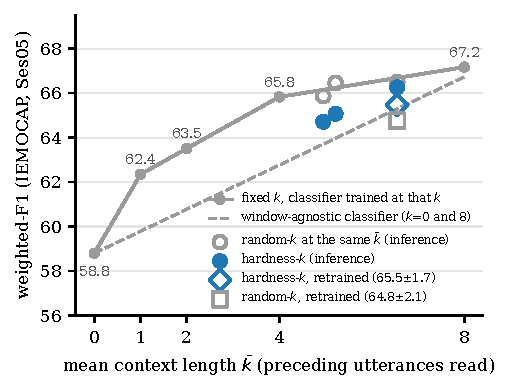
\includegraphics[width=\columnwidth]{figures/fig3_wf1_vs_kbar.pdf}
\caption{Hardness-guided context assignment does not beat random assignment at the same mean context (IEMOCAP Session~5, 6-class \wf, mean of 5 seeds). Grey line: fixed-$k$ classifiers trained at each $k$. Dashed: one window-agnostic classifier at $k = 0$ and $k = 8$. Filled blue: the same model with hardness-guided lengths at $\tau_k = 0.5, 0.7, 0.9$; hollow grey: the same model with lengths drawn at random to the same $\kbar$. Diamond and square: the two policies retrained under their own assignment (Table~\ref{tab:policies}).}\label{fig:curve}
\end{figure}

Fig.~\ref{fig:curve} isolates criterion (a) of the decision rule with one trained model. Filled blue points are the window-agnostic classifier evaluated with hardness-guided lengths at $\tau_k = 0.5, 0.7, 0.9$ ($\kbar = 4.95, 5.22, 6.55$); hollow grey circles are the same model with lengths drawn at random to the same $\kbar$. Hardness-guided assignment is below random at every $\tau$ ($64.7$ vs $65.9$, $65.1$ vs $66.5$, $66.3$ vs $66.5$). With both policies retrained under their own assignment (Table~\ref{tab:policies}) the order reverses but the difference stays inside noise: hardness-$k$ $65.47 \pm 1.65$ against random-$k$ $64.76 \pm 2.05$ at the same $\kbar$, paired-bootstrap CI of (random $-$ hardness) $[-2.9, +2.1]$. The dev split chose $\tau_k = 0.9$---the setting closest to ``read everything''---for all five attention-head seeds (four of five with the GRU head). Retraining the classifier under its own policy ($65.5 \pm 1.7$) does not close the gap to the fixed 8-turn model ($67.2 \pm 0.8$; paired-bootstrap CI of the difference $[+0.1, +3.3]$ in favour of fixed $k = 8$). The posterior-entropy policy behaves the same way ($65.1 \pm 2.1$). Criterion (a) is therefore not met: hardness-guided context is statistically indistinguishable from random assignment at the same mean context, and it neither saves context at equal accuracy nor adds accuracy at equal context relative to the fixed window.

On MELD the picture is simpler: no context policy, fixed or adaptive, is distinguishable from $k = 0$. The GRU hardness-$k$ row ($62.91 \pm 0.53$) is the highest MELD number in the paper, but it is $0.25$ above GRU fixed $k = 8$ and $0.4$ above attention $k = 0$, both inside one standard deviation; the inference curve for MELD (released CSVs) shows hardness-$k$ and random-$k$ within $0.3$ of each other at every $\tau$. The speaker-independent LOSO replication on IEMOCAP preserves the context effect ($57.7 \rightarrow 62.1$) at a lower absolute level, as expected for unseen speakers.

\subsection{Context gain stratified by hardness}\label{sec:strat}
This is the paper's central measurement. On IEMOCAP the benefit of context is not uniform: the easiest quartile of test utterances by $h$ gains $+4.8$ \wf{} from eight turns of context, the hardest gains $+11.2$, and the two middle quartiles sit between at $+9.8$ and $+8.2$---a rising trend, not a strictly monotone one, since Q2 and Q3 are within seed noise of each other (Table~\ref{tab:strat}, Fig.~\ref{fig:quartile}). Because the easiest quartile also has the least headroom, Table~\ref{tab:strat} adds the relative error reduction, $(\text{\wf}_{k=8} - \text{\wf}_{k=0})/(100 - \text{\wf}_{k=0})$: 14.9\% in Q1 against 19--23\% in Q2--Q4, so the pattern is not an artefact of ceiling. On MELD, where context is worth nothing overall, it is worth nothing in every quartile ($-0.9$ to $+0.3$). The hardness score therefore identifies \emph{which} utterances a context model will help---on a corpus where context helps---without reading any label.

\begin{table}[t]\centering\footnotesize\setlength{\tabcolsep}{3pt}
\caption{Test \wf{} by hardness quartile (pooled over 5 seeds). Quartiles are rank-based on $h$ within the test set; RER = relative error reduction from $k=0$ to $k=8$.}\label{tab:strat}
\begin{tabular}{llcccccc}\toprule
Corpus & Q & $\bar h$ & $k{=}0$ & $k{=}8$ & gain & RER & hard.-$k$ \\ \midrule
IEMOCAP & Q1 & 0.28 & 67.64 & 72.46 & $\mathbf{+4.82}$ & 14.9\% & 72.13 \\
IEMOCAP & Q2 & 0.49 & 57.63 & 67.40 & $+9.77$ & 23.1\% & 64.70 \\
IEMOCAP & Q3 & 0.58 & 57.73 & 65.95 & $+8.22$ & 19.4\% & 64.86 \\
IEMOCAP & Q4 & 0.74 & 52.17 & 63.32 & $\mathbf{+11.15}$ & 23.3\% & 60.48 \\ \midrule
MELD & Q1 & 0.39 & 68.54 & 67.68 & $-0.86$ & $-2.7\%$ & 66.61 \\
MELD & Q2 & 0.57 & 63.78 & 63.66 & $-0.12$ & $-0.3\%$ & 63.53 \\
MELD & Q3 & 0.66 & 60.12 & 60.14 & $+0.02$ & $0.1\%$ & 60.05 \\
MELD & Q4 & 0.79 & 57.59 & 57.94 & $+0.35$ & $0.8\%$ & 55.63 \\ \midrule
EmoryNLP & Q1 & 0.27 & 47.27 & 47.88 & $+0.61$ & $1.2\%$ & 48.65 \\
EmoryNLP & Q2 & 0.50 & 30.99 & 30.59 & $-0.40$ & $-0.6\%$ & 31.84 \\
EmoryNLP & Q3 & 0.61 & 31.70 & 31.25 & $-0.45$ & $-0.7\%$ & 31.19 \\
EmoryNLP & Q4 & 0.72 & 31.45 & 31.19 & $-0.26$ & $-0.4\%$ & 30.83 \\ \bottomrule
\end{tabular}
\end{table}

\begin{figure*}[t]\centering
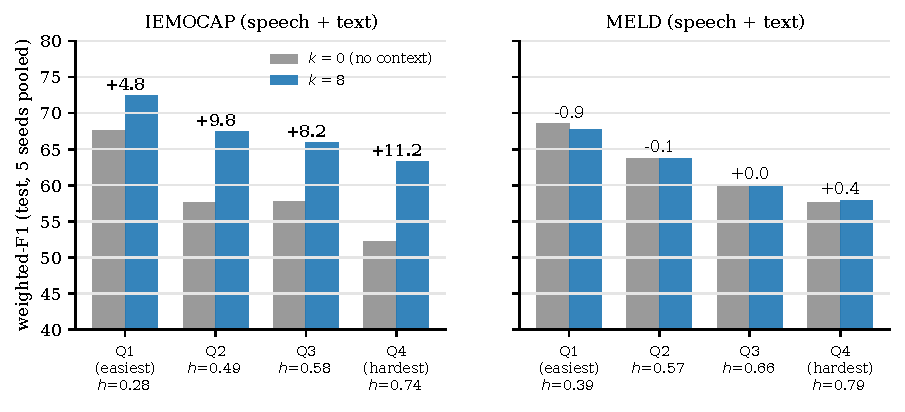
\includegraphics[width=\textwidth]{figures/fig4_gain_by_quartile.pdf}
\caption{Context gain grows with hardness on IEMOCAP ($+4.8$ to $+11.2$ \wf) and is absent on MELD. Test \wf{} by hardness quartile; grey = no context ($k = 0$), blue = eight preceding utterances ($k = 8$); the label is the gain. Fixed-$k$ models, 5 seeds pooled.}\label{fig:quartile}
\end{figure*}

Three features of Fig.~\ref{fig:quartile} matter for the rest of the paper. First, $h$ orders difficulty on every corpus: $k = 0$ \wf{} falls from $67.6$ to $52.2$ across IEMOCAP quartiles and from $68.5$ to $57.6$ across MELD quartiles, which is what a label-free hardness score should do. Second, the \emph{gain} of context is ordered by $h$ only on IEMOCAP; MELD's flat profile is not a failure of $h$ but a property of the corpus, consistent with every fixed window in Table~\ref{tab:policies}. Third, the hardness-$k$ policy column is below $k = 8$ in every IEMOCAP quartile, including the two hardest where criterion (a) required the gain to concentrate---the policy reads \emph{less} context exactly where context is worth most.

\begin{table}[t]\centering\footnotesize\setlength{\tabcolsep}{3pt}
\caption{Oracle of sufficient context $k^*$ by hardness quartile (training folds; \% of utterances). \emph{Unres.} = never classified with margin $> 0.10$ at any $k$.}\label{tab:oracle}
\begin{tabular}{llccccccc}\toprule
Corpus & Q & unres. & $k^*{=}0$ & 1 & 2 & 4 & 8 & $\overline{k^*}$ \\ \midrule
IEMOCAP & Q1 & 35.1 & 42.4 & 5.5 & 4.9 & 5.2 & 7.0 & 1.41 \\
IEMOCAP & Q2 & 38.8 & 39.3 & 4.4 & 5.0 & 4.3 & 8.1 & 1.58 \\
IEMOCAP & Q3 & 41.6 & 36.1 & 4.5 & 4.3 & 5.4 & 8.3 & 1.72 \\
IEMOCAP & Q4 & 43.7 & 32.2 & 5.0 & 4.8 & 5.4 & 8.9 & 1.90 \\ \midrule
MELD & Q1 & 37.2 & 56.5 & 1.4 & 1.4 & 1.4 & 2.0 & 0.41 \\
MELD & Q2 & 39.8 & 53.6 & 1.4 & 1.8 & 1.4 & 2.0 & 0.44 \\
MELD & Q3 & 42.3 & 51.0 & 1.3 & 1.9 & 1.3 & 2.3 & 0.50 \\
MELD & Q4 & 46.1 & 46.3 & 1.4 & 2.5 & 1.5 & 2.2 & 0.55 \\ \bottomrule
\end{tabular}
\end{table}

The oracle is monotone in $h$ on both corpora---unresolvable $35 \rightarrow 44\%$ and $k^*{=}0$ $42 \rightarrow 32\%$ on IEMOCAP, $37 \rightarrow 46\%$ and $57 \rightarrow 46\%$ on MELD---and it is bimodal everywhere: on IEMOCAP 77--79\% of training utterances are either resolved with no context or resolved by none, and only 21--24\% have a sufficient context length strictly between. Section~\ref{sec:discussion} returns to this distribution as the reason a per-utterance policy cannot win.

\begin{table}[t]\centering\small
\caption{Per-class F1 on IEMOCAP Session~5 (pooled over 5 seeds), and the row-normalised confusions (\% of the true class) that context changes most.}\label{tab:perclass}
\begin{tabular}{lccccccc}\toprule
Config. & ang & hap & neu & sad & exc & fru & \wf \\ \midrule
fixed $k=0$ & 61.9 & 30.0 & 62.8 & 67.7 & 61.0 & 56.9 & 58.8 \\
fixed $k=8$ & 65.0 & \textbf{41.2} & 70.6 & 76.2 & \textbf{72.6} & 64.6 & 67.2 \\
hardness-$k$ & 61.9 & 41.2 & 69.6 & 74.8 & 69.5 & 63.1 & 65.5 \\ \bottomrule
\end{tabular}
\vspace{4pt}
\begin{tabular}{lcc}\toprule
True $\rightarrow$ predicted & $k=0$ & $k=8$ \\ \midrule
happy $\rightarrow$ neutral & 30.5 & 17.9 \\
happy $\rightarrow$ excited & 29.1 & 35.5 \\
excited $\rightarrow$ neutral & 18.0 & 11.4 \\
frustrated $\rightarrow$ neutral & 22.0 & 15.1 \\
sad $\rightarrow$ neutral & 15.0 & 7.0 \\
frustrated $\rightarrow$ angry & 15.9 & 15.9 \\
angry $\rightarrow$ frustrated & 20.1 & 25.7 \\ \bottomrule
\end{tabular}
\end{table}

Context helps every class, most of all the two low-arousal-ambiguous ones (Table~\ref{tab:perclass}): \emph{happy} ($+11.2$ F1) and \emph{excited} ($+11.6$), whose confusion with \emph{neutral} falls from 30.5\% and 18.0\% to 17.9\% and 11.4\%. What context resolves on IEMOCAP is above all the \emph{X $\rightarrow$ neutral} confusion---every emotional class loses 6--13 points of leakage into \emph{neutral}---while the two pairs that human evaluators also confuse, \emph{happy}/\emph{excited} and \emph{angry}/\emph{frustrated}, are not resolved by context and even grow slightly ($29.1 \rightarrow 35.5\%$, $20.1 \rightarrow 25.7\%$). This is consistent with Section~\ref{sec:conf}: the classifier's residual errors after context are the pairs where the labels themselves are unstable, and neither context nor $h$ addresses them.

\subsection{Ablations, cross-corpus transfer and compact variants}
None of the hardness-conditioned design choices matters: on IEMOCAP every ablation of the gate, the head and the sign of the curriculum weight lies within one standard deviation of the default, and every paired-bootstrap interval contains zero (Table~\ref{tab:ablation}). The one exception is $\lambda = -1$ on MELD, where de-emphasising hard utterances costs $1.2$ \wf.

\begin{table*}[t]\centering\footnotesize\setlength{\tabcolsep}{3pt}
\caption{Ablations under the hardness-$k$ policy (\wf, mean $\pm$ std, 5 seeds). $\Delta$ = paired-bootstrap 95\% CI of (row $-$ default) on IEMOCAP.}\label{tab:ablation}
\begin{tabular}{lcccc}\toprule
Variant & IEMOCAP & $\Delta$ (IEMOCAP) & MELD & EmoryNLP \\ \midrule
default (FiLM, MLP, attention, $\lambda = 0.5$) & $65.47 \pm 1.65$ & 0 & $61.40 \pm 1.06$ & $35.42 \pm 0.89$ \\
gate: scalar concat $[z; h]$ & $65.96 \pm 0.39$ & $[-0.7, +2.1]$ & $62.43 \pm 0.43$ & $33.35 \pm 0.53$ \\
gate: random ($h$ permuted, matched marginal) & $65.75 \pm 0.77$ & $[-2.3, +2.3]$ & $61.32 \pm 0.82$ & $34.45 \pm 0.79$ \\
gate: none & $65.76 \pm 0.70$ & $[-2.5, +2.7]$ & $61.61 \pm 0.47$ & $34.16 \pm 0.78$ \\
head: 1-D conv instead of MLP & $66.45 \pm 1.75$ & $[-1.2, +3.1]$ & $61.64 \pm 0.87$ & $34.33 \pm 0.69$ \\
context: BiGRU instead of attention & $64.25 \pm 1.05$ & $[-2.7, +0.3]$ & $62.91 \pm 0.53$ & $35.43 \pm 0.57$ \\
$\lambda = -1$ (de-emphasise hard) & $64.88 \pm 1.14$ & $[-3.0, +1.9]$ & $60.24 \pm 0.88$ & $35.32 \pm 0.70$ \\
$\lambda = -0.5$ & $65.75 \pm 1.21$ & $[-1.5, +1.7]$ & $61.23 \pm 0.83$ & $34.76 \pm 0.85$ \\
$\lambda = 0$ (plain cross-entropy) & $65.84 \pm 1.09$ & $[-2.2, +2.2]$ & $61.67 \pm 0.64$ & $34.90 \pm 0.64$ \\
$\lambda = +1$ (emphasise hard) & $65.72 \pm 0.80$ & $[-2.0, +2.4]$ & $61.51 \pm 0.72$ & $34.59 \pm 0.72$ \\
acoustic: wav2vec2-base instead of WavLM-Large & $61.95 \pm 2.7$ & & $61.10 \pm 0.3$ & --- \\
text: MiniLM-L6 instead of RoBERTa-base & $62.52 \pm 2.0$ & & $57.40 \pm 0.8$ & $32.22 \pm 0.7$ \\ \bottomrule
\end{tabular}
\end{table*}

The random-gate control is the decisive row: a gate fed a permuted $h$ performs exactly like the real one ($65.75$ vs $65.47$ on IEMOCAP, $61.32$ vs $61.40$ on MELD), so whatever the FiLM gate contributes it is not information in $h$. The encoder rows are the only large effects in the table and they are not about hardness: WavLM-Large over wav2vec2-base is worth $+3.5$ \wf{} on IEMOCAP and nothing on MELD; RoBERTa-base over MiniLM-L6 is worth $+3.0$ on IEMOCAP and $+4.0$ on MELD. Replacing RoBERTa-base (125\,M) by MiniLM-L6 (22\,M) costs $3.0$ \wf{} on IEMOCAP, $4.0$ on MELD and $3.2$ on EmoryNLP; the head is three orders of magnitude smaller than either encoder, so inference cost is the encoders'.

\begin{table}[t]\centering\small
\caption{Cross-corpus transfer on the 4-class common set \{angry, happy, neutral, sad\} (\wf, 3 seeds). Train on one corpus, test on the other.}\label{tab:cross}
\begin{tabular}{lcc}\toprule
Train $\rightarrow$ Test & $k = 0$ & $k = 8$ \\ \midrule
MELD $\rightarrow$ IEMOCAP & 45.65 & 49.51 \\
IEMOCAP $\rightarrow$ MELD & 40.38 & 39.05 \\ \bottomrule
\end{tabular}
\end{table}

The cross-corpus asymmetry (Table~\ref{tab:cross}) mirrors the within-corpus result: a context model trained on MELD still extracts $+3.9$ \wf{} from context when tested on IEMOCAP dialogues, while a model trained on IEMOCAP gains nothing from MELD context. The direction of the effect is a property of the test dialogues, not of the training corpus.

\subsection{Hardness as a confidence signal and as an estimate of annotator disagreement}\label{sec:conf}
$h$ is a weak confidence signal and no estimate of human ambiguity (Table~\ref{tab:conf}). Pooled over seeds on the default configuration: $h$ correlates with test error at $\rho = 0.09$--$0.11$, far below the model's own posterior entropy ($0.33$--$0.36$), and adds only $0.04$--$0.06$ of partial correlation once entropy is known. As a rejection signal $h$ is worse than model confidence on every corpus (AURC $35.0$ vs $26.3$ on IEMOCAP, $31.0$ vs $20.7$ on MELD) and does not improve on confidence when added to it.

\begin{table}[t]\centering\footnotesize\setlength{\tabcolsep}{3pt}
\caption{Calibration, selective prediction and correlation with human disagreement (default configuration, pooled over 5 seeds).}\label{tab:conf}
\begin{tabular}{lccc}\toprule
 & IEMOCAP & MELD & EmoryNLP \\ \midrule
Test error rate (\%) & 40.7 & 35.7 & 59.0 \\
ECE (15 bins, \%) & 7.8 & 4.9 & 8.6 \\
$\rho(h, \text{error})$ & 0.106 & 0.093 & 0.112 \\
$\rho(\text{entropy}, \text{error})$ & 0.329 & 0.355 & 0.220 \\
$\rho(h, \text{model entropy})$ & 0.155 & 0.153 & 0.241 \\
partial $\rho(h, \text{error} \mid \text{entropy})$ & 0.059 & 0.041 & 0.062 \\
AURC, reject by confidence & 26.3 & 20.7 & 47.8 \\
AURC, reject by $h$ & 35.0 & 31.0 & 52.7 \\
AURC, reject by confidence $+ h$ & 27.3 & 23.1 & 47.8 \\
Error (\%), lowest / highest $h$-decile & 26 / 45 & 26 / 40 & 44 / 65 \\
Test utt.\ with three votes ($\times$5 seeds) & 1{,}622 (8{,}110) & --- & --- \\
$\rho(h, \text{disagreement})$ & \textbf{0.036} & & \\
$\rho(\text{entropy}, \text{disagreement})$ & 0.105 & & \\
partial $\rho(h, \text{disagreement} \mid \text{entropy})$ & \textbf{0.020} & & \\ \bottomrule
\end{tabular}
\end{table}

Criterion (b) of the decision rule required partial $\rho(h, \text{disagreement} \mid \text{entropy}) \geq 0.15$ on IEMOCAP; the observed value is $0.02$, and even the raw correlation is $0.04$. The hypothesis that neighbourhood label entropy in a frozen embedding space tracks what human evaluators disagree about is rejected on this corpus. Two observations qualify the result without rescuing it. First, nothing in our system tracks disagreement well---the model's own entropy reaches only $0.105$---so IEMOCAP's evaluator disagreement, which Busso et al.~\cite{busso2008iemocap} report as frequent between the \emph{frustrated}/\emph{angry} and \emph{happy}/\emph{excited} pairs, is largely orthogonal to the classifier's uncertainty. Second, $h$ does order error: the error rate rises from 26\% in the lowest $h$-decile to 45--49\% in the highest on IEMOCAP, and from 26\% to 40--45\% on MELD. $h$ is a coarse, label-free difficulty ranking---useful for stratifying a result table (Section~\ref{sec:strat}), not for deciding whether a single prediction should be trusted.

\section{Discussion}\label{sec:discussion}
\textbf{Why hardness predicts who benefits from context but cannot drive a per-utterance policy.} Tables~\ref{tab:strat} and~\ref{tab:oracle} together give the mechanism. Across hardness quartiles the share of utterances that need \emph{no} context falls ($42 \rightarrow 32\%$) and the share that are \emph{never} resolved rises ($35 \rightarrow 44\%$), while the share with a sufficient context length strictly between 0 and 8 stays at 21--24\%. The hardest quartile therefore gains most from a fixed window ($+11.2$) because it contains the fewest utterances that were already right and because a long window rescues some of the rest, not because its utterances have a characteristic context length that a predictor could learn. The quantity a per-utterance policy needs---``how many turns will make \emph{this} utterance right''---is bimodal and only weakly ordered by $h$; the quantity $h$ provides---``how mixed is the local label neighbourhood''---orders difficulty. The predictor $g$ learns exactly this: its most frequent outputs are $k^*{=}0$ and \emph{unresolvable}, the dev split pushes $\tau_k$ to 0.9, and the realised policy is ``read everything'' for 53--66\% of utterances and short windows for the rest. Reading short windows for the rest is where it loses to the fixed window, since the fixed window loses nothing on the utterances that did not need it ($k = 8$ is at or above $k = 0$ in every IEMOCAP quartile).

\textbf{The matched-random control is what settles it.} Without Fig.~\ref{fig:curve} the hardness-$k$ row of Table~\ref{tab:policies} could be read as a near miss: $65.5$ vs $67.2$ with overlapping seeds. With it, and with the trained random-$k$ row of Table~\ref{tab:policies} ($64.8 \pm 2.1$ against $65.5 \pm 1.7$, CI spanning zero), the policy is seen to be no better than drawing context lengths at random with the same mean. We think this control---absent from every adaptive-context ERC paper we know of---should become standard; a policy that cannot beat it has learned nothing about \emph{which} utterances need context, whatever its headline number.

\textbf{Why MELD and IEMOCAP differ.} On MELD no window length changes \wf{} by more than seed noise, audio adds $1.9$, and the oracle says 46--57\% of utterances need no context in every quartile. MELD's utterances are short sitcom lines with laugh-track audio and a 47\% \emph{neutral} majority; its emotional information is largely local. IEMOCAP's dyadic improvisations carry emotion across turns, and the cross-corpus result (Table~\ref{tab:cross}) confirms that the effect belongs to the test dialogues: a MELD-trained model still gains from IEMOCAP context, an IEMOCAP-trained model gains nothing from MELD context. A context mechanism reported as a single average over IEMOCAP and MELD is, in our setting, averaging an effect of about eight \wf{} with one of about zero; per-corpus reporting is the minimum.

\textbf{What $h$ is good for.} Three uses survive this study. (i)~Stratified reporting: a hardness-quartile table costs nothing, needs no labels at test time, and turns a single \wf{} into a profile of where a method gains---Table~\ref{tab:strat} is the first such profile for context in ERC. (ii)~Deciding whether a corpus rewards context before building a context model: the $k^*{=}0$ share of the oracle, or more cheaply the gain profile on a frozen-feature probe, separates IEMOCAP from MELD in a few GPU-minutes. (iii)~Difficulty-aware error analysis: error rises from 26\% to 45--49\% across $h$-deciles on both multimodal corpora, so $h$ is a label-free way to find the slices on which a system fails. What $h$ is not good for---per-prediction confidence, ambiguity estimation and per-utterance context selection---the preceding sections have shown.

\textbf{Relation to the pre-specified rule.} The decision rule in Section~\ref{sec:rule} was written after a text-only pilot in which the context effect was null on all three corpora. The multimodal runs produced the context effect the hypothesis needed (IEMOCAP $+8.4$) and the stratification it predicted (Table~\ref{tab:strat}), and then failed the two criteria that would have made it a method. We regard the stratified gain as the paper's positive finding and the two failures as findings of equal standing; their value to the field is that the baselines that produced them (random-$k$ at matched $\kbar$, oracle $k^*$, partial correlation given model entropy) are now specified and released.

\section{Limitations}\label{sec:limits}
\emph{Encoders are frozen.} All results concern a frozen WavLM-Large + RoBERTa-base feature space; a fine-tuned encoder could change both the absolute numbers and the hardness geometry. The frozen setting was chosen so that every effect is attributable to the context mechanism and so that the embeddings could be released; it is also the setting in which the published adaptive-context claims we test were made.

\emph{The oracle is relative to our classifier.} $k^*$ is the smallest window at which \emph{our} fixed-window head is confidently right; a stronger classifier would resolve some \emph{unresolvable} utterances. The oracle was computed at one margin threshold ($\tau = 0.10$) with the attention head; a sensitivity analysis over $\tau$ and over the head was not run, and is the first thing a reader who doubts the bimodality should run with the released code.

\emph{One policy family.} We tested a predictor of sufficient context trained on the oracle, with two heads, three thresholds and a retraining pass, plus a posterior-entropy policy. A reinforcement-learned or test-time-adaptive policy is not excluded by our results, but it would have to beat the same matched-random control.

\emph{Corpora.} IEMOCAP is acted, English and dyadic; MELD is scripted television; EmoryNLP is text only. Our conclusion that the context effect is corpus-specific is itself evidence that these three do not span conversational emotion. MELD is not speaker-independent and we say so; IEMOCAP's primary split is speaker-independent and the LOSO replication agrees with it.

\emph{Disagreement data.} The annotator-disagreement test uses IEMOCAP's three-evaluator votes; MELD and EmoryNLP release no per-annotator labels, so criterion (b) was testable on one corpus only.

\emph{No interaction study.} Earlier revisions planned a rater study of a confidence-aware response policy. Because $h$ was found not to carry confidence information beyond the model's own entropy (Section~\ref{sec:conf}), the study was not run; building it on $h$ would have tested a signal this paper shows to be empty.

\section{Conclusion}\label{sec:conclusion}
We set out to build hardness-aware context selection for multimodal ERC and committed in advance to the evidence that would justify the claim. The evidence did not arrive, and the pre-specified rule is what allows us to say so cleanly. What did arrive is, we believe, more useful than a one-point improvement would have been: a label-free hardness score that stratifies ERC evaluation; the first measurement showing that the gain from conversational context on IEMOCAP rises with hardness ($+4.8$ \wf{} in the easiest quartile, $+11.2$ in the hardest) while on MELD it is zero at every level; an oracle of sufficient context showing that the distribution a per-utterance policy must predict is bimodal---roughly 40\% need nothing, 40\% are beyond reach---which is why a learned policy is indistinguishable from random assignment at matched mean context and trails a fixed 8-turn window; and the demonstration that neighbourhood label entropy in a self-supervised embedding space does not track human disagreement. The practical recommendations are short: use a fixed window as long as the corpus rewards, test whether it rewards one before designing around it, and report context gains by hardness quartile against a matched-random control. Code, cached embeddings and per-seed results are released so that each of these recommendations can be checked.

\section*{Reproducibility}
Released with the paper: the Colab notebook that produced every number (\texttt{hardness\_aware\_ERC\_final\_colab.ipynb}, rev.~4c), the cached WavLM-Large / RoBERTa-base / MiniLM / wav2vec2 embeddings for the three corpora, per-seed result CSVs for every configuration, pooled test predictions, the oracle $k^*$ arrays, and the superseded results of the text-only pilot and of the mismatched-policy run, so that the history described in Sections~\ref{sec:rule} and~\ref{sec:discussion} can be audited. IEMOCAP and MELD are distributed under their own licences and are not redistributed. \TODO{Repository URL and embedding DOI to be inserted at submission.}

\bibliographystyle{IEEEtran}
\bibliography{references}

\begin{IEEEbiographynophoto}{Sudipta Bhattacharya}
(Member, IEEE) received the Ph.D. degree in computer science and engineering from GIET University in 2023 and the M.Tech. degree from IIEST Shibpur. He is an Associate Professor in the Department of CSE (AIML) and CSBS, Institute of Engineering and Management, Kolkata, India, and a member of the IEM Centre of Excellence for Cloud Computing and IoT. His research interests include speech emotion recognition, multilingual and low-resource speech processing, and music information retrieval.
\end{IEEEbiographynophoto}

\end{document}
